\documentclass[pmlr]{jmlr}% new name PMLR (Proceedings of Machine Learning Research)

 % The following packages will be automatically loaded:
 % amsmath, amssymb, natbib, graphicx, url, algorithm2e

 %\usepackage{rotating}% for sideways figures and tables
\usepackage{longtable}% for long tables

 % The booktabs package is used by this sample document
 % (it provides \toprule, \midrule and \bottomrule).
 % Remove the next line if you don't require it.
\usepackage{booktabs}
 % The siunitx package is used by this sample document
 % to align numbers in a column by their decimal point.
 % Remove the next line if you don't require it.
\usepackage[load-configurations=version-1]{siunitx} % newer version
 %\usepackage{siunitx}
 
 % OG from doc https://en.wikibooks.org/wiki/LaTeX/Tables#Floating_with_table 
 \usepackage{multirow}

 % The following command is just for this sample document:
\newcommand{\cs}[1]{\texttt{\char`\\#1}}

 % Define an unnumbered theorem just for this sample document:
\theorembodyfont{\upshape}
\theoremheaderfont{\scshape}
\theorempostheader{:}
\theoremsep{\newline}
\newtheorem*{note}{Note}

 % change the arguments, as appropriate, in the following:
\jmlrvolume{1}
\jmlryear{2010}
\jmlrworkshop{Workshop Title}

\title[SLAPI]{Simultaneous Localization and Active Phenomenon Inference (SLAPI)}

 % Use \Name{Author Name} to specify the name.

 % Spaces are used to separate forenames from the surname so that
 % the surnames can be picked up for the page header and copyright footer.
 
 % If the surname contains spaces, enclose the surname
 % in braces, e.g. \Name{John {Smith Jones}} similarly
 % if the name has a "von" part, e.g \Name{Jane {de Winter}}.
 % If the first letter in the forenames is a diacritic
 % enclose the diacritic in braces, e.g. \Name{{\'E}louise Smith}

 % *** Make sure there's no spurious space before \nametag ***

 % Two authors with the same address
  \author{\Name{Olivier L. Georgeon} \Email{ogeorgeon@univ-catholyon.fr}\\
  \addr UR Confluence, Sciences et Humanités (EA 1598) - Lyon Catholic University, France\\
  \Name{Titouan Knockaert} \Email{titouan.knockaert@gmail.com}\\
  \addr Université Claude Bernard Lyon 1, LIRIS CNRS UMR5205, F-69622 Villeurbanne, France\\
  \Name{Juan Vidal} \Email{jvidal@univ-catholyon.fr}\\
  \addr UR Confluence, Sciences et Humanités (EA 1598) - Lyon Catholic University, France
}


\editor{Editor's name}
 % \editors{List of editors' names}

\begin{document}

\maketitle

\begin{abstract}
We introduce the problem for a robot to  localize itself, and, simultaneously, actively infer the existence and properties of \textit{phenomena} present in its surrounding environment: the SLAPI problem. 
A phenomenon is a representation of an entity ``as the robot experiences it'' through interaction. 
The SLAPI problem relates to the SLAM problem but differs in that it does not aim at constructing a precise map of the environment, and it can apply to robots with coarse sensors. 
We demonstrated a SLAPI algorithm to control a robot equipped with omni-directional wheels, an echo-localization sensor, photosensitive sensors, and an inertial measurement unit, but no precise sensors like camera, lidar, or odometry. 
As the robot circles around an object, it constructs the phenomenon corresponding to this object under the form of the set of the spatially-localized control loops of interaction that the object affords to the robot. 
SLAPI algorithms could help design pet robots that mimic intrinsic motivation such as curiosity and playfulness with toys. 
Further studies of the SLAPI problem could improve the scientific understanding of how cognitive beings construct knowledge about objects from sensorimotor experience of interaction.
\end{abstract}

\begin{keywords}
Constructivist learning; active inference; autonomous robotics, SLAM
\end{keywords}

\section{Introduction}
\label{sec:intro}

The problem of getting mobile robots to autonomously learn the position of surrounding objects, recognize them, and keep track of their relative displacements is considered by many to be a key prerequisite of truly autonomous robots. 
Within this framework, the SLAM problem (Simultaneous Localization and Mapping) has been formalized and studied since the 1990s: constructing and updating a map of an unknown environment while simultaneously keeping track of the robot's position within it \citep[e.g.,][]{taketomi_visual_2017}.
SLAM algorithms are tailored to the available resources: odometric sensors, sensors of the environment, computational capacities, as well as the landmarks' properties, quantity, and dynamics, and the usage intended for the robot.

When displacements are imprecise and odometric data is not available, when landmarks are not directly identifiable, and below a certain level of scarcity and noise in the sensory data relative to the environment’s complexity, it becomes difficult to perform SLAM accurately enough to use the robot for tasks involving complex navigation \citep{gay_towards_2021}. 
For such robots, we propose the SLAPI problem:  Simultaneous Localization and Active Phenomenon Inference.
In contrast with SLAM, SLAPI does not aim at constructing a map to use for navigation. 
Instead, it aims at organizing behavior spatially in the vicinity of objects to design robots that mimic intrinsic motivation such as playfulness and curiosity as they discover and interact with unknown objects \citep[e.g.,][]{oudeyer_intrinsic_2007}. 
Possible applications may not include delivery tasks but may include entertainment and games, similar to playing with pets. 

SLAPI makes no assumption that landmarks can be directly and passively uniquely identified through sensors. 
The robot must rather actively interact with objects, possibly from different angles and through different modalities of control loops, to categorize and recognize objects, and possibly use them as landmarks. 
We call this process \textit{active phenomenon inference}, in line with the theory of active inference \cite[e.g.,][]{friston_world_2021}. 
% Here the term \textit{phenomenon} refers to the knowledge of physical objects actively constructed by the robot from its point of view and ``as the robot experiences the object through interaction'' \citep{thorisson_explanation_2021}. 


\section{The representational status of sensory data}
\label{sec:input}

An autonomous agent faces the necessity to actively infer the existence and the properties of objects in its environment when such existence and properties are not directly registered in sensory data. 
This raises the question of the \textit{representational status of sensory} data: is sensory data representational or not? 
This question has been discussed times and again at the philosophical level \citep[e.g.,][]{williford_husserls_2013}.
Loosely, two hypotheses collide: the hypothesis that sensory data carry information about features of the world, versus the hypothesis that sensory data carry information about the agent's experience of interaction with the world. 
We refer to the former as the \textit{representationalist hypothesis}, and to the latter as the \textit{constructivist hypothesis} because it relates to Piaget's theory of construcitivist learning based on sensorimotor schemes \citep{guillermin_artificial_2022}. 

SLAPI falls within the constructivist hypothesis because it applies to robots that have coarse sensors that do not provide much descriptive information about the environment. 
The robot must probe the environment a little bit like a blind person who uses a cane to actively construct a mental representation of its surroundings. 
Probing experiences consist of control loops during which the robot interacts with the environment.   
They are triggered by an action selected by the robot and result in an outcome. 
The outcome is informative not of the object itself but of the possibility of interaction afforded by the object to the robot. 
Past probing experiences drive future behavior because they constitute affordances for action. 
\figureref{fig:cycle} shows this cycle of interaction. 
The software selects an action associated with spatial information that specify how the control loop should be enacted in the world. 
In return, the software receives an outcome associated with spatial information that describes how the control loop has been enacted depending on the actual nature and position of surrounding objects. 


\begin{figure}[htbp]
	% Caption and label go in the first argument and the figure contents
	% go in the second argument
	\floatconts
	{fig:cycle}
	{\caption{The interaction cycle. Black bullet: the cycle begins with the software selecting an action containing spatial information to enact in the world (right). Black arrowhead: the cycle ends with the software receiving the outcome containing spatial information (left).}}
	{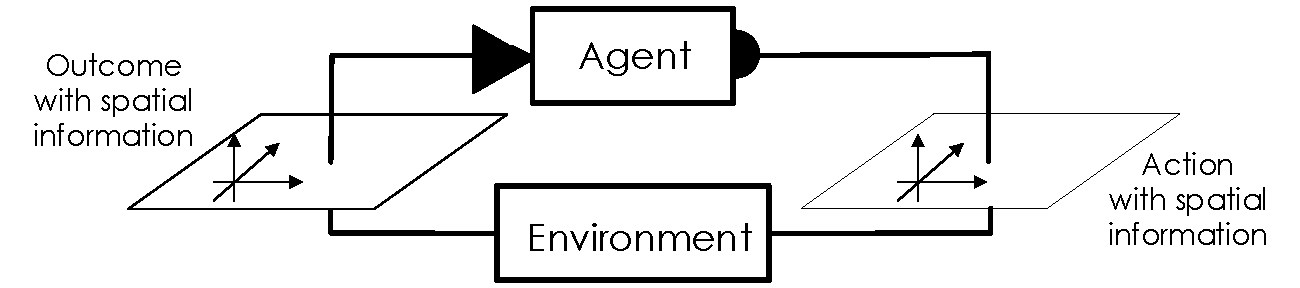
\includegraphics[width=0.8\linewidth]{images/Figure_0_Cycle}}
\end{figure}

Note that the constructivist hypothesis accepts that the outcome may sometimes register features of the environment but only avoids ``baking'' this assumption in the algorithm \textit{a priori}. 
\cite{rudrauf_mathematical_2017} have also proposed an active inference model related to the constructivist hypothesis. He states that ``All we need here is the idea that in one way or another the sensory organs provide an independent source of input and correction for the continually updated world model'' (p. 19).


\section{The experimental setup}
\label{sec:experiment}

We use the robot cat of brand Osoyoo\footnote{\url{https://osoyoo.com/2019/11/08/omni-direction-mecanum-wheel-robotic-kit-v1/}}, to which we added an inertial measurement unit (\figureref{fig:robot}). 
We set up an environment with black lines on the floor and various objects that can be detected through the echo-localization sensor. 
There is not final target to reach. We only want the robot to explore its environment. 

\begin{figure}[htbp]
	% Caption and label go in the first argument and the figure contents
	% go in the second argument
	\floatconts
	{fig:robot}
	{\caption{The experimental setup. 
			Osoyoo robots, a black line on the floor, and various objects detectable through echo-localization.
		    The omni-directional wheels allow the robot to translate laterally (sweep right or left).}}
	{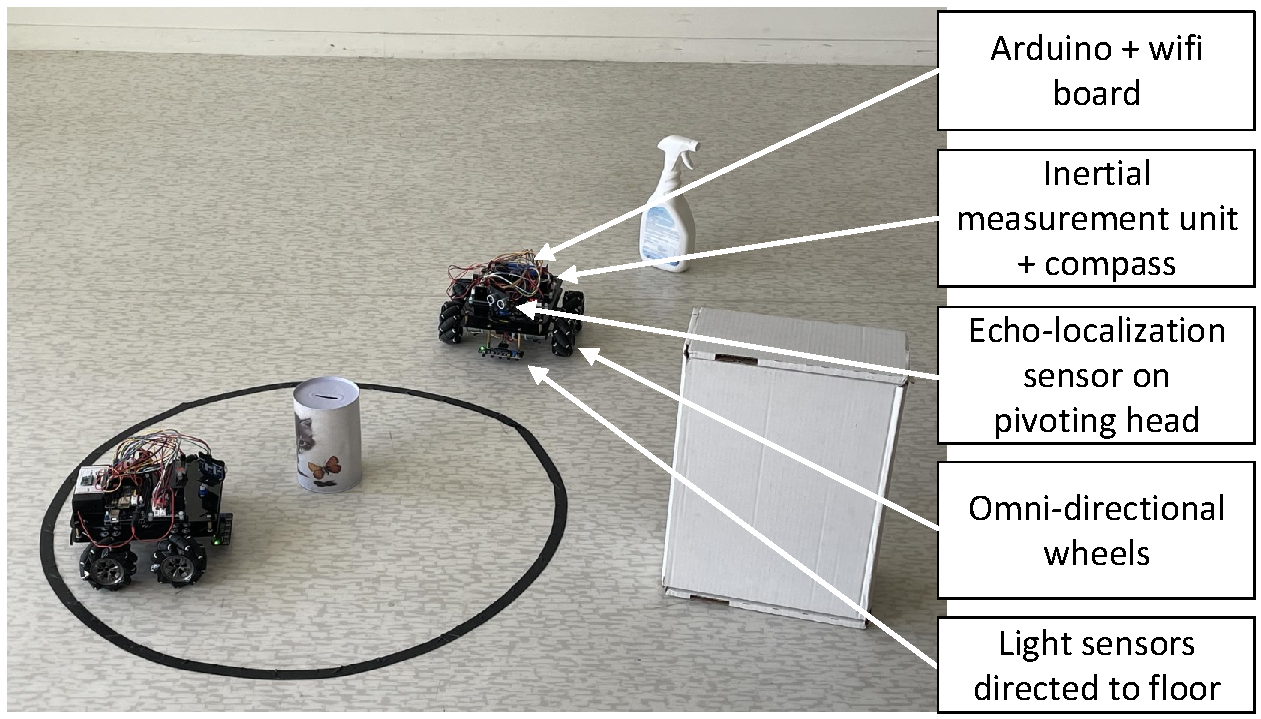
\includegraphics[width=0.8\linewidth]{images/Figure_1_Robotb}}
\end{figure}


\section{The software architecture and algorithm}
\label{sec:software}

We implemented the cognitive architecture on a remote PC as depicted in \figureref{fig:architecture}. 
This architecture takes the place of the \textit{Software} in \figureref{fig:cycle}, whereas the robot plus its environment takes the place of the \textit{World}.

The architecture follows a regular Model-View-Controller design pattern in which the \textit{Memory} plays the role of the database, and the \textit{Workspace} plays the role of the Model. 
As we will further develop, the \textit{Memory} contains the Egocentric memory and the Allocentric memory which are displayed on screen via the \textit{View Controllers} (\figureref{fig:architecture}, right).
The \textit{Workspace} contains the \textit{Decider} which implements the robot's policy, and the \textit{Synthesizer} which infers the phenomena. 

\begin{figure}[htbp]
	% Caption and label go in the first argument and the figure contents
	% go in the second argument
	\floatconts
	{fig:architecture}
	{\caption{The software architecture implemented on a remote PC. 
			Bottom: the robot recieves the action and sends back the outcome through wifi.
			Top-right: Egocentric memory shows the position of echos (orange circles), the focus of attention (red hexagon), and the previous positions of the robot (green triangles).
			Bottom-right: Allocentric memory shows the position of the echo (orange cells), the explored cells (white), the position of the robot (green), the unexpored cells (grey).}}
	{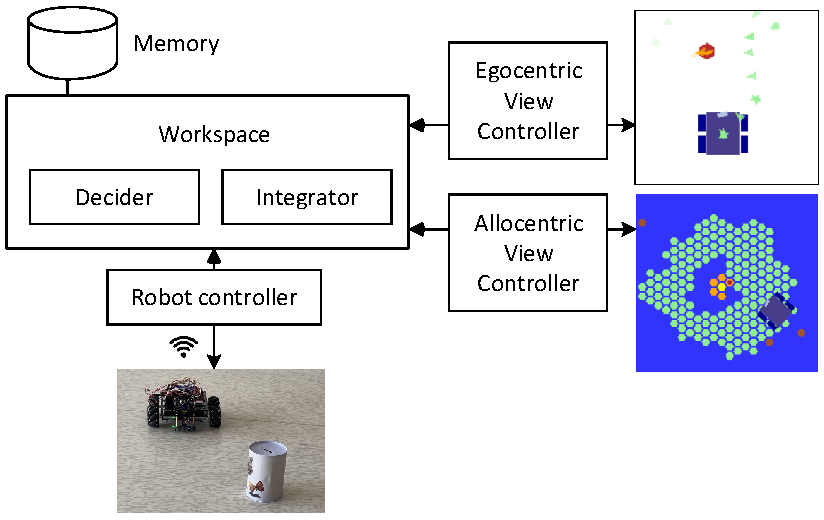
\includegraphics[width=0.8\linewidth]{images/Figure_2_Architecture}}
\end{figure}


\subsection{The control loops of interaction implemented in the robot}

A C++ program on the robot's Arduino board handles the reception of the action, drives the control loop, and then returns the outcome through wifi. 
\tableref{tab:action} lists the supported actions and outcomes.

The reception of an action triggers the enaction of the corresponding control loop until its termination condition.
For example, the \texttt{Forward} action sets the robot in motion. 
It has three possible termination conditions: 
\texttt{Default}: time out of 1 second (approximately 20 cm traveled);
\texttt{Line detection}: the floor sensor detects a line causing the robot to retreat back for a few centimeters; and
\texttt{Shock}: the inertial measurement unit detects a strong deceleration indicating a shock against an object.


\begin{table}[htbp]
	\floatconts
	{tab:action}
	{\caption{Actions available to the robot and their possible outcomes}}
	{%
		\subtable[Actions]{%
			\label{tab:ab}%
			\begin{tabular}{lc}
				\toprule
				\bfseries Code & \bfseries Description\\
				\midrule
				\texttt{Forward} & \multirow{4}{2.5cm}{During 1 sec. or until shock or line detection}\\
				\texttt{Backward} &  \\
				\texttt{Sweep left} &  \\
				\texttt{Sweep right} & \\ \hline
				\texttt{Turn left} & $\pi/4$ \\
				\texttt{Turn right} & $-\pi/4$ \\ \hline
				\texttt{Head scan} & $[-\pi/2, \pi/2]$ \\
				\bottomrule
		\end{tabular}}
		\qquad
		\subtable[Outcomes]{%
			\label{tab:cd}%
			\begin{tabular}{lc}
				\toprule
				\bfseries Code & \bfseries Description\\
				\midrule
				\texttt{Line left} & \multirow{3}{2.8cm}{Floor sensors cross luminosity threshold } \\
				\texttt{Line front} & \\
				\texttt{Line right} & \\ \hline
				\texttt{Shock} & Violent deceleration \\ \hline
				\texttt{Echo lost focus} & No echo where expected \\ \hline
				\texttt{Echo left} & \multirow{6}{3cm}{Direction and range of the nearest echo}\\  
				\texttt{Echo right} &  \\  
				\texttt{Echo far left} & \\  
				\texttt{Echo far right} & \\  
				\texttt{Echo far front} & \\
				\texttt{Echo close front} & \\ \hline
				\texttt{Default} & No line, no echo \\ 
				\bottomrule
			\end{tabular}
		}
	}
\end{table}

Besides the action code, the cognitive architecture sends two more values to the robot: the coordinates of a focus point, and an estimated speed. 
The robot's program uses these to keep the robot's head aligned towards the focus point during the robot's displacement. 
This helps the robot keep tracks of objects over various moves. 
It also gives the human observer the impression that the robot keeps it attention to a particular object, making it look more alive. 

The robot also returns additional information to the cognitive architecture: the yaw, azimuth (angle relative to the north) and duration of the various phases of the control loop. 
The cognitive architecture uses this information to update the spatial memory based on the robot's displacement. 
The termination phase of the control loop aligns the robot's head towards the nearest echo. 
The robot then returns the nearest echo measure along with the head direction. 
The cognitive architecture uses this information to mark the position of the echo in spatial memory. 
This will be used to infer the presence of an object in the area. 
\tableref{tab:dialogue} summarizes the data exchanged between the PC and the robot.

\begin{table}[htbp]
	% The first argument is the label.
	% The caption goes in the second argument, and the table contents
	% go in the third argument.
	\floatconts
	{tab:dialogue}%
	{\caption{Dialogue between the PC and the robot through wifi}}%
	{\begin{tabular}{l|l}
			\toprule
			PC to Robot & Action code, focus coordinates $(x, y)$, estimated speed $(x, y)$\\
			\midrule
			Robot to PC & Outcome code, echo distance, head direction, yaw, azimuth, duration\\
			\bottomrule
	\end{tabular}}
\end{table}

\subsection{The egocentric memory}

The egocentric memory is a short-term memory of the experiences of interaction in the surrounding of the robot. 
It is inspired by the brain's egocentric cells located in the superior colliculus \citep{grieves_representation_2017}.

Technically, it stores the robot's \textit{experiences} in a coordinate system centered on the robot.
An experience is a data structure that contains the action, the outcome, the position in space relative to the robot, and the timestamp. 
Our implementation initializes the position in space from a hard-coded model of the robot: line-detection experiences are placed at the position of the floor sensors; echo experiences are placed at the estimated origin of the echo using head direction and measure of echo distance.  
When the robot moves, the positions of experiences are then moved opposite by the robot's estimated displacement (\figureref{fig:architecture}, top right). 
Of course, errors accumulate causing a drift in egocentric memory. 
With our robot, we observed that the position of experiences were unreliable after 5 to 10 interaction cycles.


\subsection{The allocentric memory}

The allocentric memory stores a spatial representation in a coordinate system relative the environment. 
It is inspired by \textit{grid cells} in the hippocampus of the mammalian brain \citep{grieves_representation_2017}.

Our implementation reproduces the grid cell's hexagonal structure (\figureref{fig:architecture}, bottom right). 
Each cell stores the list of experiences enacted in the location referenced by the cell, and can have one of the following status:

\begin{altdescription}{Phenomenon}
	\item[Unknown] No experience has been attempted here.
	\item[Occupied] The robot is localized here.
	\item[Empty] The robot has been here in the past.
	\item[Experience] One or several experiences have been localized here.
\end{altdescription}

Allocentric memory is used to construct a local spatial representation of the objects with which the robot is interacting.
It keeps track of the robot's position through path integration. 
It informs the next action to select by the \textit{Decider}, and constitutes the base for phenomenal inference performed by the \textit{Synthesizer}. 

\subsection{The decider}
\label{sec:decider}

The Decider implements the policy that selects the action for the robot to enact. 
There is an nascent literature on how to model an information-seeking policy inspired by animal behavior \citep[e.g.,][]{gottlieb_towards_2018}.
The choice and the implementation of such policy is a part of the SLAPI problem. 

Here we propose a proof of concept based upon a cognitive architecture that we have implemented previously \citep{georgeon_eca_2013}.
The cognitive architecture stores a \textit{list of behaviors} in the form of \textit{sequences of experiences} that the robot can enact. 
After each interaction cycle, the decider searches this list and activates the sequence of experience whose beginning sub-sequence matches experiences present in memory. 
The activated behaviors then propose their ending sub-sequences for further enaction. 
Finally the decider selects the continuing sub-sequence that is proposed with the highest weight. 

In the present study, we have initialized the list of behaviors with predefined behavioral patterns that give the robot a tendency to circle around objects when it detects them. 
The robot wanders randomly until it detects an object nearby, and then it circles around this object until the experimenter removes the object. 


\subsection{The synthesizer}
\label{sec:synthesizer}


Once an object has been identified in allocentric memory, the synthesizer copies its representation to a data structure called a \textit{phenomenon}.

We use the term phenomenon in its common sense: the perception by a cognitive beeing of ``something'' in the environment.
In computer science, we comply with \cite{thorisson_explanation_2021}'s definition of ``Any useful grouping of a subset of spatio-temporal patterns experienced by an agent in an environment''.

In our implementation, the phenomenon data structure stores a local map of experiences afforded by the object. 
This map is a subset of egocentric memory converted to a coordinate system centered on the phenomenon.
This process of phenomenon inference is performed by the Synthesizer.

The synthesizer constructs a representation of an object by reading experiences from egocentric memory and filling and updating allocentric memory. 
It works in coordination with the Decider (\sectionref{sec:decider}) to explore the object through different directions. 

It infers the presence of an object from repeated experiences in the same area. 
Once an object has been identified with enough experiences, it can be isolated in allocentric memory and copied to a phenomenon data structure.

\section{Results}

\figureref{fig:results} reports two different phenomena constructed from two kinds of object: an object that affords echo and shock (top), and an object that also affords line detection (bottom).
A representative run can be seen in video \citep{titouan_knockaert_demonstration_2022}.
It shows the robot circling around the object while constructing the egocentric and allocentric maps. 
It is worth noting that many human observers attribute the intention of the robot to carefully observe the object due to the fact that it keeps its head pointing to the object. 

\begin{figure}[htbp]
	% Caption and label go in the first argument and the figure contents
	% go in the second argument
	\floatconts
	{fig:results}
	{\caption{Examples of phenomenon inference.
			  Left: the robot and the object seen by the human observer.
			  Right: the phenomenon constructed by the robot. 
			  Top: the object affords echo (orange cells) and shock (red cells). 
			  Bottom: the object also affords line detection (black cells). 
			  Green cells represent empty space.}}
	{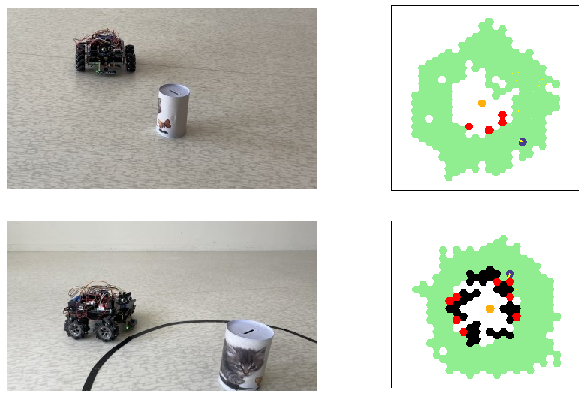
\includegraphics[width=0.6\linewidth]{images/Figure_3_results}}
\end{figure}


\section{Conclusion}

This paper presents the SLAPI problem: the problem for an autonomous artificial agent to construct knowledge about entities in its environment from sensorimotor experience of interaction.  
This problem is particularly salient when the agent has rudimentary sensors that provide poor information about the features of the environment. 
In this case, to be informative, sensory data should rather be considered as \textit{outcome} of a control loop than \textit{percepts}.

On the contrary, when the agent has rich sensors that allow the identification of features of the world, it is tempting for the developer of the agent's software to consider that sensory data carries representational information about the world. 
Philosophy of mind, however, provide theoretical arguments against this representationalist hypothesis. 
These arguments go back to Kant, who claimed that the world ``in itself'' is unknowable, and relate to Piaget's developmental psychology and constructivist epistemology. 
They also have echos in modern physics. 
If we trust these arguments, we can expect SLAPI algorithms to also bring value to agents that have rich sensors. 
They could endow such agents with more autonomy in the way they construct their own knowledge of the world, and keep this knowledge grounded in their individual experience of interaction.

We reported our implementation and experiment as an initial example to illustrate the SLAPI problem, in the hope that it provides clarification. 
We hope that future algorithms will address more complex problems of phenomenal inference, such as categorization and recognition of similarities and differences between types of phenomena. 
In return, we hope that such studies can inform research in neuroscience on how animals construct knowledge of objects through their experience of interaction.

\bibliography{olivier}


\end{document}
